% !TEX root = deckblatt4.tex
\section{Messung eines Rechtecksignals}
\subsection{Aufgabenstellung}
Hier sollte ein Rechtecksignal in Zeit und Frequnenzbereich gemessen werden und anschlie\ss{}end die Ergebnisse erl\"autert werden

\subsection{Vorbereitung \& Messaufbau}
Es wurde mit dem Frequnezgenerator ein Rechtecksingal mit einer Amplitude von $1V_{pp}$ und einer Frequnez von $10kHz$ erzeugt. Der Ausgang des Frequnezgenerators wurde direkt mit dem Tastkopf des Oszilloskops verbunden, es wurde keine Messschaltung aufgebaud.

\begin{figure}[H]
 \begin{center}
  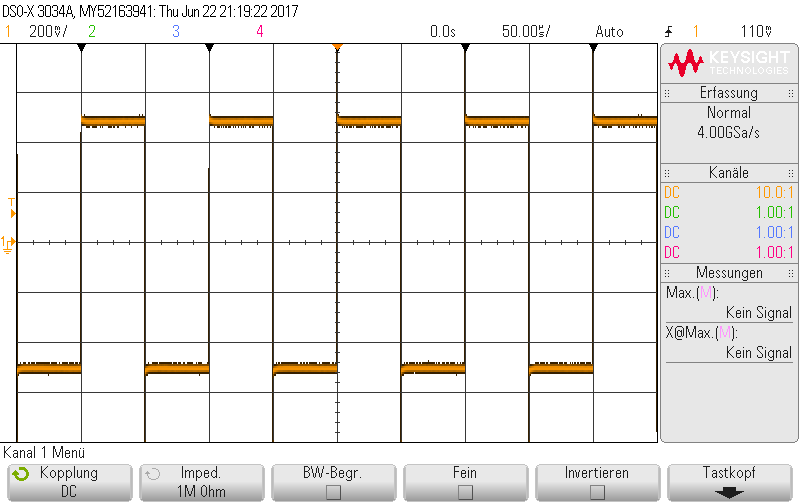
\includegraphics[height=6cm,width=12cm]{OsziBilder/bsp2_time.png}
 \end{center}
 \caption{Rechteckspannung $1V_{pp}$, $10kHz$}\label{bsp2_time}
\end{figure}
\noindent
In Abbildung \ref{bsp2_time} ist, dass Rechtecksignal, welches zur Messung verwendet wurde im Zeitbereich zu sehen. \\
\newpage

\subsection{FFT}
In dieser Messung wurde das Hanning-Fenster verwendet, da dies ein sehr einfaches und g\"angiges Fenster ist.

\begin{figure}[H]
 \begin{center}
  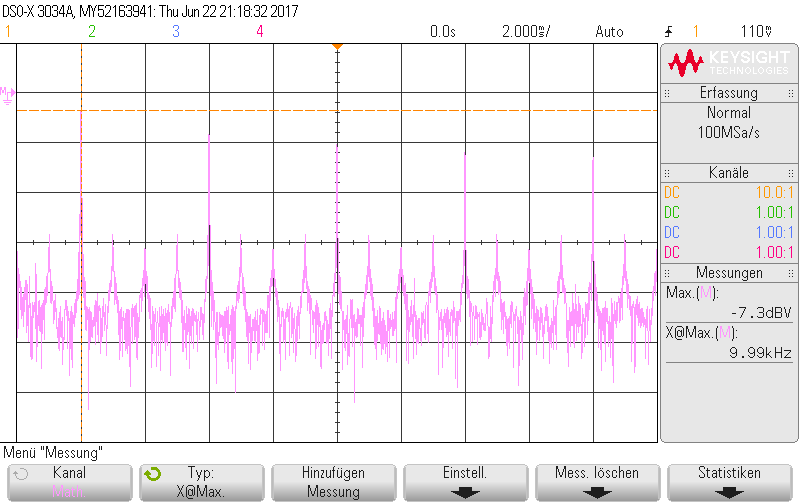
\includegraphics[height=6cm,width=12cm]{OsziBilder/bsp2_Hanning_dB.png}
 \end{center}
 \caption{Rechteckspannung $1V_{pp}$, $10kHz$}\label{bsp2_dB}
\end{figure}
\noindent

\begin{figure}[H]
 \begin{center}
  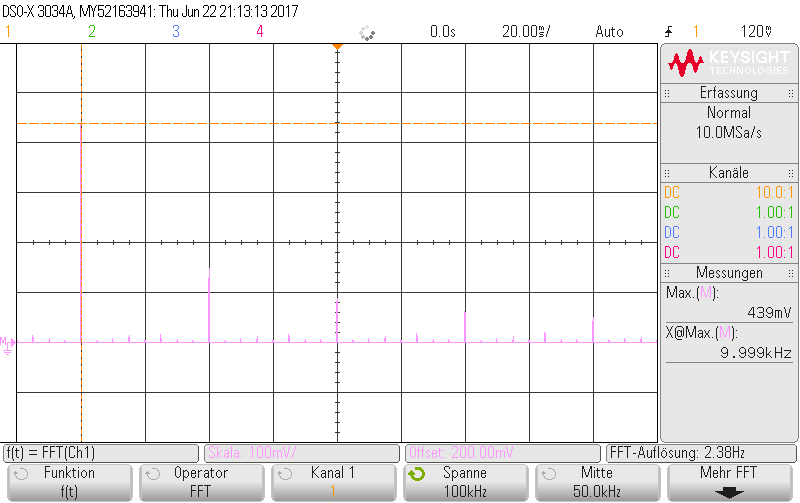
\includegraphics[height=6cm,width=12cm]{OsziBilder/bsp2_Hanning_RMS_Cursor.png}
 \end{center}
 \caption{Rechteckspannung $1V_{pp}$, $10kHz$}\label{bsp2_rms}
\end{figure}
\noindent
In den beiden Abbildungen \ref{bsp2_dB} \& \ref{bsp2_rms} sind die Spektren des oben gezeigten Rechecksignals zu sehen. In Abbildung \ref{bsp2_dB} wurde f\"ur die y-Achse eiene Logarithmische dB Skalierung verwendet und in Abbildung \ref{bsp2_rms} eine lineare. \\
In den Beiden Abbildungen ist der der Vorteil der dB - Skalierung deutlich zu erknnen. W\"ahrend in Abbildung \ref{bsp2_dB} die Amplitude bei $90kHz$ nur um etwar $10dB$ kleiner als die der Grundfrequnez, so ist diese in der Linearen Darstellung schon verschwindend gering. \\
Wie erwartet stechen bei einem Symetrischen Rechteck alle Ungeraden Vielfachen der Grundfrequnez hervor.

\begin{figure}[H]
  \begin{center}
    \begin{tabular}{|c|c|} \hline
    $f_g=10kHz$ & $439mV$ \\ \hline
    $3*f_g$ & $147,11mV$ \\ \hline
    $5*f_g$ & $90,77mV$ \\ \hline
    $7*f_g$ & $62,60mV$ \\ \hline
    \end{tabular}
  \end{center}
  \caption{Messwerte der Hauptkomponente und der ersten 3 Nebenkomponenten}
\end{figure}
\noindent
In obiger Tabelle sind die Amplitden zu der Grundrequnez und den ersten drei ungeraden Vielfachen herausgemessen worden. Man kann sehr gut erkennen, dass die Werte exponentiell kleiner werden. 
